\chapter{Systematic uncertainties}\label{chap:systematics}
Systematic uncertainties need to be taken into account because of the
imperfect knowledge of either detector effects or theory.
Detector effects include uncertainties in the trigger efficiencies, the
efficiency of the lepton reconstruction, the jet energy correction factors
and pile-up conditions.

Lepton reconstruction efficiencies were studied in~\cite{CMS-EXO-12-001}. The uncertainty on the trigger
efficiency is taken to be 5\%. This is a conservative estimate based on the study of the dilepton triggers in~\cite{bprime2011}. We also include a 2.2\% uncertainty 
on the luminosity~\cite{CMS-SMP-12-008}. These systematic uncertainties are summarized in Table~\ref{tab:Systematics}.

\begin{table}
    \centering
\begin{tabular}{*2c}
    \toprule
          effect & uncertainty (\%) \\
          \midrule
  electron trigger          & 5.0 \\
  muon trigger              & 5.0 \\
  lepton efficiency         & 3.0 \\
  luminosity                & 2.2 \\
  \bottomrule
\end{tabular}
\caption{Systematic uncertainties.}
\label{tab:Systematics}
\end{table}

\section{Monte Carlo systematics}
The jet energy scale (JES) and pile-up uncertainties are calculated by
varying the JES and pile-up according to the recommended recipes in the samples for which 
we take the result from Monte Carlo. The JES and pile-up uncertainties for the backgrounds are 
summarized in Table~\ref{tab:MConlySystematics}. For the signal points, we
take the JES and pile-up uncertainties to be the maximum value of these for single
point. This corresponds to 0.9\% for the JES and 2\% for the pile-up. Table~\ref{tab:MConlySystematics} also
contains the overall normalization uncertainty for each background sample.

The $\W\Z$ and $\Z\Z$ normalization uncertainties are taken from~\cite{CMS-AN-2011-333}. 
For the rare backgrounds, we assume a normalization uncertainty of 50\%, as
these processes have never been observed at the LHC or have not been
measured well.

\begin{table}[htb]
    \centering
\begin{tabular}{*4c}
    \toprule
    sample       &    jet energy & pile-up & normalization \\
    \midrule
$\W\Z$             & 5.0\%  & 1.8\%  & 17\%    \\
$\Z\Z$             & 1.1\%  & 0.6\%  & 7.5\% \\
$\W^{\pm}\W^{\pm}$ & 4.5\%  & 2.4\%  & 50\% \\
$\W\W\W$            & 3.7\%  & 0.5\%  & 50\% \\
$\ttbar \W$       & 3.4\%  & 0.94\% & 50\% \\
$\ttbar \Z$       & 3.7\%  & 0.25\% & 50\% \\
\bottomrule
\end{tabular}
\caption{Systematic uncertainties for backgrounds that are taken from Monte Carlo.}
\label{tab:MConlySystematics}
\end{table}

\section{Data-driven background systematics}
We also include a 50\% uncertainty associated with the
estimation of the non-prompt lepton background~\ref{sec:closure}
and a 20\% uncertainty for the charge misidentification. This comes from the
difference between the expected number of events derived with the method
described in~\ref{sec:charge_misid} and a more sophisticated $\eta$
dependent estimate. We can see that the charge misidentification probability
depends on $\eta$ (figure~\ref{fig:charge_misid_eta}), and is lower in the
barrel with respect to the endcaps.
\begin{figure}[htb]
    \centering
    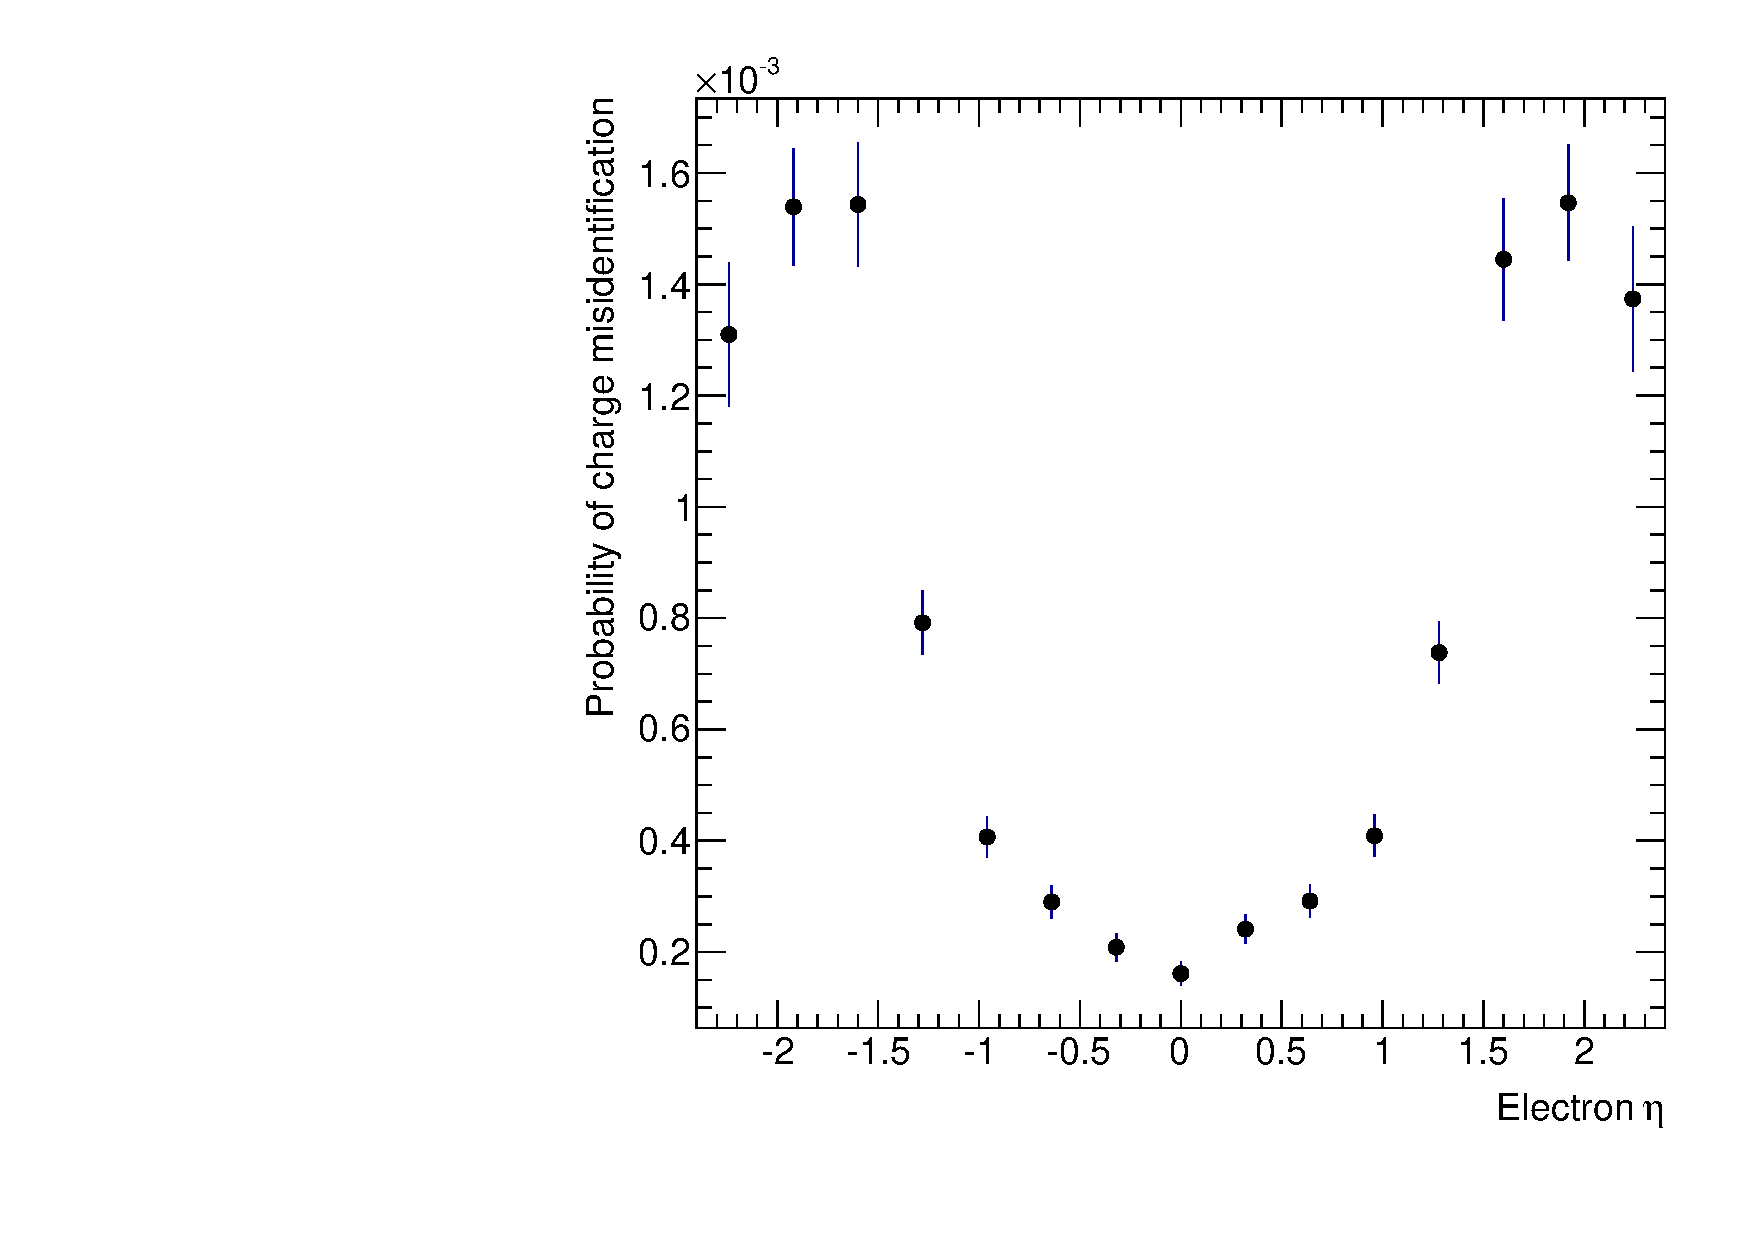
\includegraphics[width=.7\textwidth]{images/pdf/h_MisIDProbvsEta}
    \caption{Charge misidentification probability as a function of the
    pseudorapidity $\eta$.}
    \label{fig:charge_misid_eta}
\end{figure}
However, given the very small amount of events with charge misidentification
passing our selections, this contribution to the total uncertainty is small
as well.
These uncertainties are summarized in
table~\ref{tab:data_driven_syst}.
\begin{table}[h]
    \centering
    \begin{tabular}{ll}
        \toprule
        data-driven method & uncertainty \\
        \midrule
        charge misid & 20\%\\
        non-prompt & 50\%\\
        \bottomrule
    \end{tabular}
    \caption{Systematic uncertainties for data-driven backgrounds}
    \label{tab:data_driven_syst}
\end{table}

The inputs to the calculation of the limits on the $\TP$ mass affected by the systematic uncertainties are the luminosity, the uncertainty on the signal efficiency 
and the uncertainty on the total background. The latter is the largest of
the three and it is completely dominated by the 50\% uncertainty associated with the estimation of the 
non-prompt lepton background and the normalization uncertainty on the rare backgrounds.


